\documentclass{standalone}
\usepackage{pgfplots}
\usetikzlibrary{intersections}
\pgfplotsset{compat=1.7}

\begin{document}
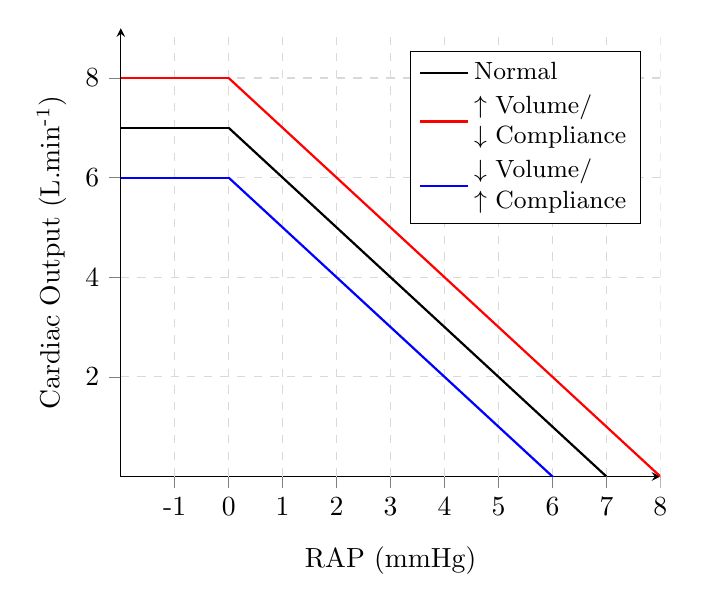
\begin{tikzpicture}


\begin{axis}[
        axis lines=middle,
        grid = major,
        grid style={dashed, gray!30},
	ymin = 0,
	ymax = 9,
	xmin = 0,
	xmax =10,
	 ylabel near ticks,
	xlabel near ticks,
	xticklabels={},
	extra x ticks={1,2,3,4,5,6,7,8,9,10},
	extra x tick labels={-1,0,1,2,3,4,5,6,7,8,9,10},
        xlabel=RAP (mmHg),
        ylabel=Cardiac Output (L.min\textsuperscript{-1}),
        tick align=outside,
        enlargelimits=false,
legend pos= north west,
legend style={font=\small, cells={align=left}, at={(0.75,0.95)},anchor=north},
legend cell align={left}]

\draw[name=vr, black, thick] (axis cs: 0, 7) -- (axis cs: 2,7);
\plot[domain=2:9, black, thick,samples=500] {9-x};
\addlegendentry{Normal}
\draw[name=vr, red, thick] (axis cs: 0, 8) -- (axis cs: 2,8);
\plot[domain=2:10, red, thick,samples=500] {10-x};
\addlegendentry{$\uparrow$ Volume/ \\ $\downarrow$ Compliance}
\draw[name=vr, blue, thick] (axis cs: 0, 6) -- (axis cs: 2,6);
\plot[domain=2:10, blue, thick,samples=500] {8-x};
\addlegendentry{$\downarrow$ Volume/ \\ $\uparrow$ Compliance}


\end{axis}

\end{tikzpicture} 
\end{document}